\documentclass[bsc,frontabs,twoside,singlespacing,parskip,deptreport]{infthesis}

\usepackage[round]{natbib}
\usepackage[hidelinks,colorlinks,allcolors=blue]{hyperref}

\usepackage{graphicx}

\usepackage{textcomp} % for text tilde

% bold in mah mode, making the needed fonts available
\usepackage{amsmath}
\usepackage{lmodern}
\usepackage{bm}

% additional keywords in math mode
\DeclareMathOperator{\softmax}{softmax}

% Nice references including the words Figure, Section, etc
\renewcommand*{\chapterautorefname}{Chapter}
\renewcommand*{\sectionautorefname}{Section}
\renewcommand*{\subsectionautorefname}{Section}
\renewcommand*{\figureautorefname}{Fig.}
\renewcommand*{\tableautorefname}{Tab.}
\newcommand{\algorithmautorefname}{Alg.}
\def\equationautorefname~#1\null{(#1)\null}

% Change font family and size in captions
\DeclareCaptionFont{captionfont}{\small\fontseries{n}\fontfamily{phv}\selectfont}
\captionsetup[table]{labelsep=period,font=captionfont,justification=centering}
\captionsetup[figure]{labelsep=period,font=captionfont,justification=centering}


%
% TABLES
%

\usepackage{multirow} % multi-row and multi-column table cells
\usepackage{makecell} % line breaks inside cells with \thead{} and \makecell{}
\usepackage{longtable} % allow table to span multiple pages

% Globally setting the vertical padding in tables
\renewcommand{\arraystretch}{1.1}

% Spacing around lines in tables
\def\abovestrut#1{\rule[0in]{0in}{#1}\ignorespaces}
\def\belowstrut#1{\rule[-#1]{0in}{#1}\ignorespaces}
\def\abovespace{\abovestrut{0.17in}}
\def\aroundspace{\abovestrut{0.17in}\belowstrut{0.10in}}
\def\belowspace{\belowstrut{0.10in}}


% For minipages with multiple figures, each with its own subcaption
\usepackage{subcaption}

% For verbatim in captions
\usepackage{cprotect}

% For verbatim in footnotes
\usepackage{fancyvrb}

\begin{document}
\VerbatimFootnotes

\title{\vspace{-5.0cm} \centering{\includeshield} \vspace{1cm} \\ Teacher-student knowledge distillation from BERT\\for sentence classifiers}

\author{Sam Su\v{c}\'ik}

\course{Master of Informatics}
\project{\vspace{3cm}{\bf MInf Project (Part 2) Report}}

\date{2020}

\abstract{
  
}

\maketitle

\section*{Acknowledgements}{
  I thank Steve Renals of University of Edinburgh and Vova Vlasov of Rasa for supervising me throughout the academic year; patiently listening to my never-ending reports and providing helpful and optimistic comments.

  Many thanks also to Ralph Tang whose work inspired this project, and to Sl\'avka He\v{z}elyov\'a who constantly supported me and motivated me to explain all of my work in non-technical stories and metaphors.
}

{
  \hypersetup{linkcolor=black}
  \tableofcontents
}

\chapter{Introduction}{
  % what's the problem, 
  \section{Motivation}{
    \begin{itemize}
      \item After the deep learning hype started, NLP went through an era of LSTMs. Since 2017, the area has been becoming dominated by Transformer models pre-trained on large unlabelled corpora.
      
      \item As newer and bigger Transformer-based models were proposed in 2018 and 2019, improving on the SOTA, it was becoming clearer that their big size and low speed was rendering them difficult to use (both train and deploy) in practice outside of research labs.
      
      \item Recently, we've seen various early attempts at making Transformers -- in particular BERT \citep{Devlin_2018} -- smaller by removing attentional heads \citep{Michel_2019}, quantisation and pruning \citep{Cheong_2019, Sucik_2019}. In terms of actually down-sizing and accelerating the models, knowledge transfer using teacher-student knowledge distillation has led to the most attractive results \citep{Mukherjee_2019,Tang_2019a,Jiao_2019,Sanh_2019}.
      
      \item However, these studies focus only on using knowledge distillation as a tool. Important questions about the nature of this technique and how it interacts with properties of the teacher and student models remain generally unexplored.
      
      \item In line with the increasing demand for explainable AI, it is desirable that, for the beginning, at least the researchers better understand the tools they use, in this case distillation of NLP knowledge from Transformer models. Indeed, such understanding is also useful for overcoming the limitations and designing new variants of this method for smaller and better classifiers.
    \end{itemize}
  }
  
  % what I tried to address, 
  \section{Aims}{
    I aim to better understand knowledge distillation by exploring its use for knowledge transfer from BERT into different student architectures on various NLP tasks.

    This can be further broken down into three aims:
    \begin{itemize}
      \item Explore the effectiveness of knowledge distillation in very different NLP tasks. To cover a broad variety of tasks, I use sentence classification datasets ranging from binary sentiment classification to 57-way intent classification to linguistic acceptability.
      \item Explore how distilling knowledge from a Transformer varies with different student architectures. I limit myself to using the extremely popular BERT model \citep{Devlin_2018} as the teacher architecture. As students, I use two different architectures: a BiLSTM, building on the successful work of Ralph Tang \citep{Tang_2019a,Tang_2019b}, and a down-scaled BERT architecture.
      \item Explore how successfully can different types of NLP knowledge and capabilities be distilled. Since NLP tasks are often possible for humans to reason about, I analyse the models' behaviour (e.g. the mistakes they make) to learn more about knowledge distillation. I also probe the models for different linguistical capabilities, inspired by previous successful probing studies \citep{Conneau_2018,Tenney_2019b}.
    \end{itemize}
  }
  
  % what I did
  \section{Contributions}{
    My actual findings. To be added later.
  }
}

% Prerequisites: define NLP abbreviation
\chapter{Background}{
  \label{ch:background}

  In this chapter, the Transformer models are introduced and set into the historical context; knowledge distillation is introduced, in particular its recent applications in NLP; and an overview of some relevant work in model understanding is given.

  % NLP (sentence classification), transformers, knowledge distillation, model understanding (probing)
  \section{NLP before Transformers}{
    \label{sec:pre-transformer-nlp}
    % NLP is all about sequences of variable lengths: sentences, sentence pairs, documents, speech segments...
    By the very nature of the natural language, its processing has always meant processing sequences of variable length: be it written phrases or sentences, words (sequences of characters), spoken utterances, sentence pairs, or entire documents.
    % NLP tasks are typically about making simple predictions about sequences: classifying sentences based on their intent or language, scoring a document's level of formality, predicting whether two sentences form a coherent question-answer pair or not, predicting the next word of a sentence...
    Very often, NLP tasks boil down to making simple decisions about such sequences: classifying sentences based on their intent or language, assigning a score to a document based on its formality, deciding whether two given sentences form a meaningful question-answer pair, or predicting the next word of an unfinished sentence.

    % Word vectors used already by \citet{Collobert_Weston_2008,Collobert_Weston_2011}, trained in unsupervised fashion. Used for various NLP tasks in a CNN.
    As early as 2008, artificial neural networks started playing a key role in NLP: \citet{Collobert_Weston_2008}\footnote{See also \citet{Collobert_Weston_2011}.} successfully trained a deep neural model to perform a variety of tasks from part-of-speech tagging to semantic role labelling.
    % Machine learning predictors are typically designed to work with fixed-size representations of inputs. Therefore, ever since the resurgence of neural networks around 2010, neural NLP has been using various models for encoding variable-length sequences into common fixed-dimensional representations.
    However, neural machine learning models are typically suited for tasks where the dimensionality of inputs is known and fixed. Thus, it comes as no surprise that NLP research has focused on developing better models that encode variable-length sequences into fixed-length representations. 
    If any sequence (e.g. a sentence) can be embedded as a vector in a fixed-dimensionality space, a simple classification model can be learned on top of these vectors.
    
    One key step in the development of neural sequence encoder models has been the idea of \textit{word embeddings}: rich, dense, fixed-length numerical representations of words. When viewed as a lookup table -- one vector per each supported word -- such embeddings can be used to ``translate'' input words into vectors which are then processed further.
    % Word2vec \citet{Mikolov_2013} made embedding learning much more efficient (and made learning the embedings the main aim!), using CBOW and skip-grams.
    \citet{Mikolov_2013} introduced an efficient and improved way of learning high-quality word embeddings: \textit{word2vec}. The embeddings are learnt as part of a larger neural network, which is trained to predict the next word given several previous words, and the previous words given the current word\footnote{These are the so-called Continuous bag-of-words (CBOW) and Skip-gram (SG) tasks, respectively.}. Such training can easily leverage large amounts of unlabelled text data and the embeddings learn to capture various properties from a word's morphology to its semantics. Released word2vec embeddings became very popular due to their easy use and performance improvements in many NLP tasks.
    \textbf{TO-DO: Add a simple illustration of learning word2vec.}

    % \textbf{(TO-DO: Maybe mention TDNNs? They kind of fit here although they process speech, not text...)}
    
    % RNN- and later LSTM-based encoder architectures were dominating the area for a long time as they were naturally suited for processing sequences of any length.
    While word embeddings were a breakthrough, they themselves do not address the issue of encoding a sequence of words into a fixed-size representation. This is where Recurrent neural networks (RNNs) \citep{Rumelhart_1986} and later their improved variant -- Long Short-Term Memory neural networks (LSTMs) \citep{Hochreiter_Schmidhuber_1997} -- come into play. Although originally proposed long ago, they became popular in NLP, and in text processing in particular, only later (see e.g. \citet{Mikolov_2010} and \citet{Graves_2013}). These recurrent encoders process one word at a time (see \autoref{fig:RNN}) while updating an internal (``hidden'') fixed-size representation of the text seen so far. Once the entire sequence is processed, the hidden representation (also called ``hidden state'') is outputted and used make a simple prediction.
    \begin{figure}[h!t]
      \centering
      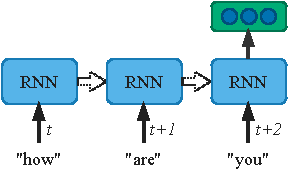
\includegraphics[width=6cm]{graphics/rnn}
      \caption{A recurrent neural network (RNN) consumes at each timestep one input word. Then, it produces a single vector representation of the inputs.}
      \label{fig:RNN}
    \end{figure}

    % A major breakthrough came when \citet{Kalchbrenner_2013} and \citet{Sutskever_2014} developed the encoder-decoder architecture for machine translation and other sequence-to-sequence tasks such as paraphrasing or parsing.
    As various recurrent models started dominating NLP, one particularly influential architecture emerged, addressing tasks such as machine translation, where the output is a new sequence rather than a simple decision. This was the \textit{encoder-decoder} architecture \citep{Kalchbrenner_2013,Sutskever_2014}, see \autoref{fig:encoder-decoder}. It uses a recurrent encoder to turn an input sentence into a single vector, and a recurrent decoder to generate an output sequence based on the vector.
    \begin{figure}[h!t]
      \centering
      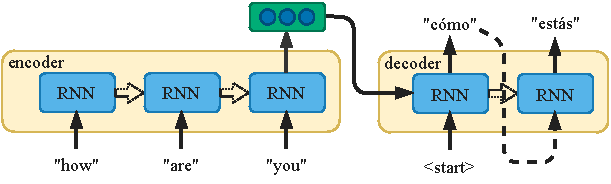
\includegraphics[width=11.5cm]{graphics/encoder-decoder}
      \cprotect\caption{An encoder-decoder model for machine translation. Notice how the decoder initially takes as input the special \verb|<start>| token and at later time consumes the previous output word.}
      \label{fig:encoder-decoder}
    \end{figure}

    % \citet{Bahdanau_2014} improved things by introducing attention, enabling the recurrent encoders to learn to selectively attend or ignore parts of the input sequence.
    \citet{Bahdanau_2014} improved encoder-decoder models by introducing the concept of \textit{attention}. The attention module helps the decoder produce better output by selectively focusing on the most relevant parts of the input at each decoder timestep. This is depicted in \autoref{fig:encoder-decoder-att}, showing the decoder just about to output the second word (``est\'as''). The steps (as numbered in the diagram) are:
    \begin{enumerate}
      \item the decoder's hidden state passed to the attention module,
      \item the intermediate hidden states of the encoder also passed to the attention module,
      \item the attention module, based on information from the decoder's state, selecting relevant information from the encoder's hidden states and combining it into the attentional \textit{context vector},
      \item the decoder combining the last outputted word (``c\'omo'') with the context vector and consuming this information to better decide which word to output next. 
    \end{enumerate}

    \begin{figure}[h!t]
      \centering
      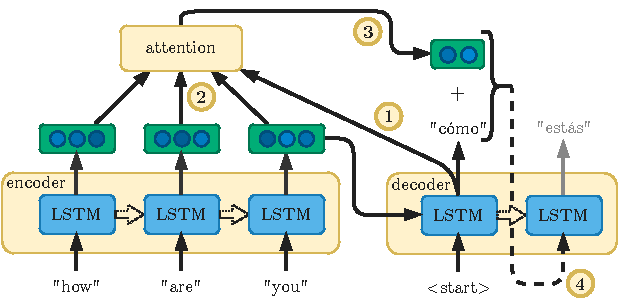
\includegraphics[width=11.5cm]{graphics/encoder-decoder-att}
      \cprotect\caption{An encoder-decoder model for machine translation with added attention mechanism.}
      \label{fig:encoder-decoder-att}
    \end{figure}
    
    The attention can be described more formally\footnote{My description does not exactly follow the original works of \citet{Bahdanau_2014} and \citet{Luong_2015}. Instead, I introduce concepts that will be useful in later sections of this work.}: First, the decoder state $\bm{h_D}$ is processed into a \textit{query} $\bm{q}$ using
    \begin{equation}
    \bm{q}=\bm{h_D}W_Q
    \end{equation}
    and each encoder state $\bm{h_{E}^{(i)}}$ is used to produce the \textit{key} and \textit{value} vectors, $\bm{k^{(i)}}$ and $\bm{v^{(i)}}$:
    \begin{equation}
    \bm{k^{(i)} = h_{E}^{(i)}W_K},\ \ \ \bm{v^{(i)} = h_{E}^{(i)}W_V}\ .
    \end{equation}
    Then, the selective focus of the attention is computed as an \textit{attention weight} $w^{(i)}$ for each encoder state \textit{i}, by combining the query with the $i$-th key:
    \begin{equation}
    w^{(i)}=\bm{q^\top}\bm{k^{(i)}}\ .
    \end{equation}
    The weights are normalised using softmax and used to create the context vector $c$ as a weighted average of the values:
    \begin{equation}
    \bm{c}=\sum_{i}a^{(i)}\bm{v^{(i)}}\ \ \ \textrm{where}\ \ \ a^{(i)}=\softmax(w^{(i)})=\frac{\exp{(w^{(i)})}}{\sum_{j}\exp{(w^{(j)})}}\ .
    \end{equation}
    Note that $W_Q$, $W_K$, $W_V$ are matrices of learnable parameters, optimised in training the model. This way, the attention's ``informed selectivity'' improves over time.
    
    For years, recurrent models with attention were the state of the art in many NLP tasks. However, as we will see, the potential of attention reached far beyond recurrent models.
  }

  \section{Transformer-based NLP}{
    \label{sec:Transformer-based-NLP}
    \subsection{Transformers}{
      \label{sec:Transformers}
      % \citet{Vaswani_2017} introduced Transformer. Main idea: process tokens in parallel, not sequentially, with sequentiality represented by positional markers (embeddings). Self-attention is used to pool from the context of the entire sequence, leading to evolving rich contextualised representations of each token in the higher layers.
      We saw how the attention mechanism can selectively focus on parts of a sequence to extract relevant information from it. This raises the question of whether processing the inputs in a sequential fashion with the recurrent encoder is still needed. In particular, RNN models are slow as a results of this sequentiality, with no room for parallelisation. In their influential work, \citet{Vaswani_2017} proposed an encoder-decoder model based solely on attention and fully parallelised: the \textit{Transformer}. The core element of the model is the \textit{self-attention} mechanism, used to process all input words in parallel.

      In particular, a Transformer model typically has multiple self-attention layers, each layer processing separate representations of all input words. Continuing with the three-word input example from \autoref{fig:encoder-decoder-att}, a high-level diagram of the workings of a self-attention layer is shown in \autoref{fig:self-att-layer}. Importantly, the input word representations evolve from lower to higher layers such that they consider not just the one input word, but also all other words -- the representation becomes \textit{contextual} (also referred to as a \textit{contextual embedding} of the word within the input sentence).

      \begin{figure}[h!t]
        \centering
        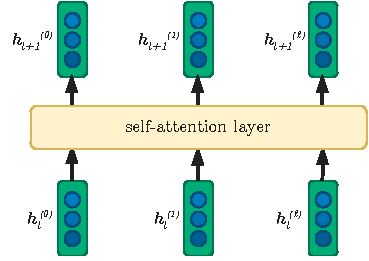
\includegraphics[width=7cm]{graphics/self-att-layer}
        \cprotect\caption{A high-level diagram of the application of self-attention in Transformer models. Three hidden states are shown for consistency with the length of the input shown in \autoref{fig:encoder-decoder-att}; in general, the input length can vary.}
        \label{fig:self-att-layer}
      \end{figure}

      As for the internals of self-attention, the basic principle is very similar to standard attention. Self-attention too is used to focus on and gather relevant information from a sequence of elements, given a query. However, to produce a richer contextual embedding $\bm{h_{l+1}^{(i)}}$ in layer $l+1$ of the $i$-th input word, self-attention uses the incoming representation $\bm{h_l^{(i)}}$ for the query, and considers focusing on all representations in layer $l$, including $\bm{h_l^{(i)}}$ itself. \autoref{fig:self-att} shows this in detail for input position $i=0$. Query $\bm{q^{(0)}}$ is produced and matched with every key in layer $l$ (i.e. $\bm{k^{(0)}},\ldots,\ \bm{k^{(2)}}$) to produce the attention weights. These weights quantify how relevant each representation $\bm{h_l^{(i)}}$ is with respect to position $i=0$. Then, the new contextual embedding $\bm{h_{l+1}^{(i)}}$ is constructed as a weighted sum of the values $\bm{v^{(0)}},\ldots,\ \bm{v^{(2)}}$ (same as constructing the context vector in standard attention).

      \begin{figure}[h!t]
        \centering
        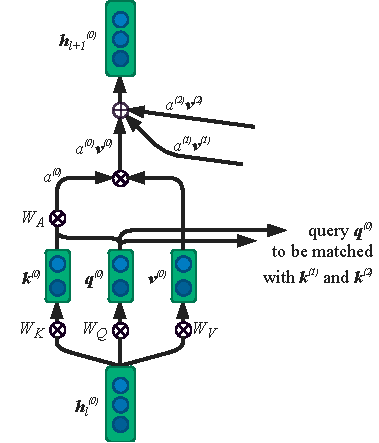
\includegraphics[width=8cm]{graphics/self-att}
        \cprotect\caption{The internals of self-attention, illustrated on creating the next-layer hidden representation of the input position $i=0$, given all representations in the current layer. Note that $\otimes$ stands for multiplication (where the multiplication involves a learnable matrix like $W_K$, this is written next to the $\otimes$), and $\oplus$ denotes summation.}
        \label{fig:self-att}
      \end{figure}

      % parallel nature
      Notice that, even though each contextual embedding considers all input positions, the next-layer contextual embeddings $\bm{h_{l+1}^{(0)}},\ldots,\ \bm{h_{l+1}^{(2)}}$ can be computed all at the same time, in parallel: First, the keys, queries and values for all input positions are computed; then, the attention weights with respect to each position are produced; finally, all the new representations are produced. It is this parallelism that allows Transformer models to run faster. As a result, they can be much bigger (and hence create richer input representations) than recurrent models while taking the same time to train.

      % positional embeddings
      Due to their parallel nature, self-attentional layers have no notion of an element's position within the input sequence. This means no sensitivity to word order. (Recurrent models sense this order quite naturally because they process input text word by word.) To alleviate this downside of self-attention, Transformers use \textit{positional embeddings}. These are artificially created numerical vectors added to each input word, different across input positions, thus enabling the model's layers to learn to be position- and order-sensitive.

      % multi-headedness
      As an additional improvement of the self-attentional mechanism, \citeauthor{Vaswani_2017} introduce the concept of multiple self-attention heads. This is very similar to having multiple instances of the self-attention module in \autoref{fig:self-att} (each instance being one \textit{head}). The motivation behind multiple self-attention heads is to enable each head $h$ to learn different ``focusing skills'' by learning its own $W_{Q,h}$, $W_{K,h}$, $W_{V,h}$. Each head produces its own output:
      \begin{equation}
      O_{att,h} = \softmax(\frac{\bm{q}\bm{k^\top}}{\sqrt{d_k}})\bm{v} = \softmax(\frac{(\bm{h_l^\top}W_{Q,h})^\top(\bm{h_l^\top}W_{K,h})}{\sqrt{d_k}})(\bm{h_l^\top}W_{V,h})
      \end{equation}
      which matches \autoref{fig:self-att} (but notice the detail of the additional scaling by $\frac{1}{\sqrt{d_k}}$, introduced by \citeauthor{Vaswani_2017}, where $d_k$ is the dimensionality of the key).
      The outputs of the $H$ individual heads are then concatenated and dimensionality reduced with a trainable linear transformation $W_{AO}$, to produce the final output, which replaces $\bm{h_{l+1}}$ in \autoref{fig:self-att}:
      \begin{equation}
      O_{att} = [O_{att, 1},\ \ldots,\ O_{att, H}]W_{AO}\ .
      \end{equation}
      
      % \citet{Radford_2018} introduced the idea of generative LM pre-training and fine-tuning. This concept helps train much better models even for low-resource tasks with small datasets, by leveraging general language knowledge acquired by the model in the pre-training phase. Publishing pre-trained model instances makes the power of NLP much more accessible to anyone and has become a popular thing to do. (Also mention that subword tokens were used instead of words.)
      Besides the self-attention-based architecture, there is one more important property that makes today's Transformer models perform so well on a wide variety of NLP tasks: the way these models are trained. First used for Transformers by \citet{Radford_2018}\footnote{The idea was previously used with recurrent models by \citet{Dai_2015}.}, the general procedure is:
      \begin{enumerate}
        \item \textit{Unsupervised pre-training}: The model is trained on one or more tasks, typically language modelling, using huge training corpora. For example, \citeauthor{Radford_2018} pre-train their model to do next word prediction (the standard language modelling task) on a huge corpus of over 7,000 books.
        \item \textit{Supervised fine-tuning}: The pre-trained model is trained on a concrete dataset to perform a desired downstream task, such as predicting the sentiment of a sentence, translating between languages, etc.
      \end{enumerate}
      This two-step procedure is conceptually similar to using pre-trained word embeddings. In both cases, the aim is to learn general language knowledge and then use this as a starting point for focusing on a particular task. However, in this newer case, the word representations learned in pre-training are be better tailored to the specific architecture, and they are inherently contextual -- compared to pre-trained word embeddings like word2vec which are typically context-insensitive. 

      Importantly, pre-trained knowledge makes models more suitable for downstream tasks with limited amounts of labelled data. The model no longer needs to acquire all the desired knowledge just from the small dataset; it contains pre-trained high-quality general language knowledge which can be reused in various downstream tasks. This means that large, powerful Transformer models become more accessible: They are successfully applicable to a wider array of smaller tasks than large models that have to be trained from scratch.
    }

    \subsection{BERT}{
      \label{sec:BERT}
      % \citet{Devlin_2018} improved the concept by pre-training the model bi-directionally (leading to language modelling based on left \textit{and} right context).
      Perhaps the most popular Transformer model today is BERT (Bidirectional Encoder Representations from Transformers), proposed by \citet{Devlin_2018}. Architecturally, it is a sequence encoder, hence suited for sequence classification tasks. While being heavily based on the original Transformer \citep{Vaswani_2017}, BERT adds a few further tricks:
      \begin{enumerate}
        \item The model learns bidirectional representations: It can be trained on language modelling that is not next-word prediction (prediction given left context), but word prediction given both the left and the right context.
        \item {It uses two very different pre-training classification tasks:
        \begin{enumerate}
          \item The \textit{masked language modelling} (MLM) task encourages BERT to learn good contextual word embeddings. The task itself is to correctly predict the token at a given position in a sentence, given that the model can see the entire sentence with the target token(s) masked out\footnote{I.e. replaced with the special \verb|[MASK]| token.}, with a different token, or left unchanged.
          \item The \textit{next-sentence prediction} (NSP) task encourages BERT to learn good sentence-level representations. Given two sentences, the task is to predict whether they formed a consecutive sentence pair in the text they came from, or not.
        \end{enumerate}
        The pre-training was carried out on text from books and from the English Wikipedia, totalling to 3,400 million words (for details see \citet{Devlin_2018}). The MLM and NSP tasks were both used throughout the pre-training, forcing the model to learn both at the same time.
        }
        \item The inputs are processed not word by word, but are broken down using a fixed vocabulary of sub-word units (\textit{wordpieces}, introduced by \citet{Wu_2016}). This way, BERT can better deal with rare words. (In word-level models, words that are not found in the model's vocabulary are replaced with a special \verb|UNKNOWN| token, which means disregarding any information carried by the words.) The tokeniser module of BERT uses the wordpiece vocabulary to tokenise (segment) the input text before it is further processed. \autoref{fig:bert-inputs} shows an example; notice how my surname (``Sucik'') gets split into three wordpieces whereas the other, much more common words are found in the wordpiece vocabulary.
        \item To enable the different pre-training tasks as well as two-sentence inputs, BERT uses a special input sequence representation, illustrated in \autoref{fig:bert-inputs}. Given the two input sentences $S_A$, $S_B$, they are concatenated and separated by the special \verb|[SEP]| token. The overall sequence is prepended with the \verb|[CLS]| (classification) token. Then, for tasks like NSP, only the output representation of the \verb|[CLS]| token (i.e. $\bm{o_0}$) is used, whereas for token-level tasks like MLM the output vector from the desired position is used (in \autoref{fig:bert-inputs}, the MLM task would use $\bm{o_3}$ to predict the correct token at this position).
      \end{enumerate}

      \begin{figure}[h!t]
        \centering
        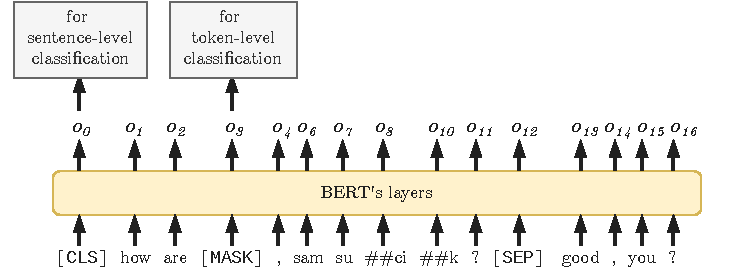
\includegraphics[width=14cm]{graphics/bert-inputs}
        \caption{BERT's handling of input for sentence-level and token-leven tasks. The input sentences ($S_A = How\ are\ you,\ Sam\ Sucik?$ and $S_B = Good,\ you?$) are shown as split by BERT's tokeniser, with the first instance of ``you'' masked out for MLM.}
        \label{fig:bert-inputs}
      \end{figure}
      % They also changed the pre-training to 2 tasks trained at the same time: masked language modelling to learn to understand words, and next sentence prediction to learn to reason about entire sentences (as the actual NLP tasks often require such reasoning). 
      % This is is how BERT was born, which then became extremely popular in the community, attracting a lot of work on improving it, analysing its capabilities, extending it to other languages, and even applying it to multi-modal tasks such as video captioning. 
      % TO-DO: elaborate more on BERT, also with a schematic picture.
      The overall architecture of BERT is shown in \autoref{fig:bert-hl}. The tokeniser also adds the special tokens like \verb|[CLS]| and \verb|[SEP]| to the input, while the trainable token embedding layer also adds positional embeddings to the tokens. The pooler takes the appropriate model output (for sequence level classification the first output $\bm{o_0}$ as discussed above) and applies a fully-connected layer with the tanh activation function.
      The external classifier is often another fully-connected layer with the tanh activation, producing the logits\footnote{For a classifier, the logits are the (unnormalised) predicted class probabilities.}. These get normalised using softmax to produce a probability distribution over all classes. The most probable class is outputted as the model's prediction.
      
      \begin{figure}[h!t]
        \centering
        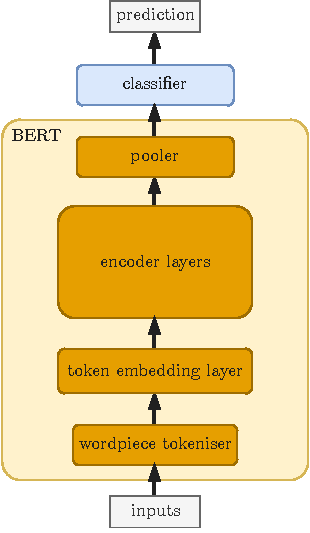
\includegraphics[width=6cm]{graphics/bert-hl}
        \caption{High-level overview of the modules that make up the architecture of BERT as used for sequence-level classification.}
        \label{fig:bert-hl}
      \end{figure}

      % things beyond what was said about Transformers already: residual connections, GeLU?
      To complete the picture of BERT, \autoref{fig:bert-encoder-layer} shows the internals of an encoder layer. Besides the multi-headed self-attention submodule, it also contains the fully-connected submodule, consisting of the intermediate fully-connected transformation with parameters $W_I$, and the layer output fully-connected transformation with parameters $W_O$. Each submodule is also by-passed by a residual connection (shown with dashed lines). The residual information is summed with the submodule's output, and layer normalisation is applied to the sum. Note that this structure is not new in BERT; it was used already by the original Transformer of \citet{Vaswani_2017}.

      \begin{figure}[h!t]
        \centering
        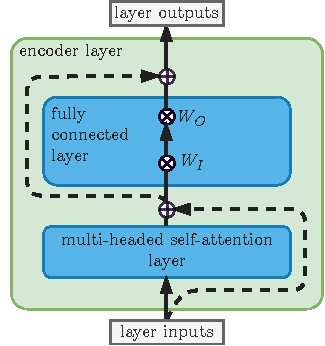
\includegraphics[width=6cm]{graphics/bert-encoder-layer}
        \caption{The modules making up one encored layer in BERT; residual connections highlighted by using dashed lines.}
        \label{fig:bert-encoder-layer}
      \end{figure}
      
      Originally, pre-trained BERT was released in two sizes: BERT\textsubscript{Base} with 110 million parameters, 12 encoder layers and 12-head self-attention, and BERT\textsubscript{Large} with 340 million parameters, 24 encoder layers and 16-head self-attention. The models quickly became popular, successfully applied to various tasks from document classification \citep{Adhikari_2019} to video captioning \citep{Sun_2019}. Further pre-trained versions were released too, covering, for example, the specific domain of biomedical text \citep{Lee_2019} or multilingual text \citep{Pires_2019}.
    }

    \subsection{Newer and larger Transformer models}{
      \label{sec:post-BERT-models}
      % Following the success of BERT, further and often bigger Transformer models started emerging:
      Following the success of the early Transformers and BERT \citep{Vaswani_2017,Radford_2018,Devlin_2018}, many further model variants started emerging, including:
      \begin{itemize}
        \item The OpenAI team releasing GPT-2 \citep{Radford_2019}, a larger and improved version of their original, simple Transformer model GPT \citep{Radford_2018}.
        \item \citep{Lample_2019} introducing XLM, which uses cross-lingual pre-training and is thus better suited for downstream tasks in different languages.
        \item Transformer-XL \citep{Dai_2019}, which features an improved self-attention that can handle very long contexts (across multiple sentences/documents).
      \end{itemize}

      All these open-sourced, powerful pre-trained models were a significant step towards more accessible high-quality NLP (in the context of downstream tasks with limited data). However, the model size -- often in 100s of million trainable parameters -- meant these models could not be applied easily in practice (outside of research): They were memory-hungry and slow.
      
      Naturally, this inspired another stream of research: Compressing large, well-performing Transformer models (very often BERT) to make them faster and resource-efficient.
      I turn my focus to one compression method that worked particularly well so far: the teacher-student knowledge distillation.
    }
  }

  \section{Teacher-student knowledge distillation}{
    \label{sec:KD}
    % brief history of KD in general
    % different objectives: logits, hard labels, mimicking internal representations...
    \subsection{A brief introduction to knowledge distillation}{
      \label{sec:KD-intro}
      Knowledge distillation was introduced by \citep{Bucila_2006} as a way of knowledge transfer from large models into small ones. The aim is to end up with a smaller -- and hence faster -- yet well-performing model. The steps are 1) to train a big neural classifier model (also called the \textit{teacher}), 2) to let a smaller neural classifier model (the \textit{student}) learn from it -- by learning to mimic the teacher's behaviour. Hence also the name \textit{teacher-student knowledge distillation}, often simply \textit{knowledge distillation}.
      
      There are different ways of defining the teacher's ``behaviour'' which the student learns to mimic. Originally, this was realised as learning to mimic the teacher's predictions: A dataset would be labelled by the teacher, and the student would be trained on these labels (which are in this context referred to as the \textit{hard labels}). The dataset used for training the student (together with the teacher-generated labels) is referred to as the \textit{transfer dataset}.

      Later, \citet{Ba_2013} introduced the idea of learning from the teacher-generated \textit{soft labels}, which are the teacher's logits. The idea is to provide the student with richer information about the teacher's decisions: While hard labels only express which class had the highest predicted probability, soft labels also describe how confident the prediction was and which other classes (and to what extent) the teacher was considering for a given example.

      When soft labels were first used, the student's training loss function was the mean squared distance between the student's and the teacher's logits:
      \begin{equation}
        E_{MSE}=\sum_{c=1}^{C}{(z_t^{(c)}-z_s^{(c)})^2}
        \label{eq:E_MSE}        
      \end{equation}
      where $C$ is the number of classes and $z_t$, $z_s$ are the the teacher's and student's logits.
      \citet{Hinton_2015} proposed a more general approach, addressing the issue of overconfident teachers with very sharp logit distributions. The issue with such distributions is that they carry little additional information beyond the hard label (since the winning class has a huge probability and all others have negligibly small probabilities).
      To ``soften'' such sharp distributions, \citeauthor{Hinton_2015} proposed using the \textit{cross-entropy loss} \autoref{eq:E_CE} in combination with softmax with temperature \autoref{eq:softmax-temperature} (instead of the standard softmax) in training both the teacher and the student.
      \begin{equation}
        E_{CE}=\sum_{c=1}^{C}{z_t^{(c)} \log{z_s^{(c)}}}
        \label{eq:E_CE}        
      \end{equation}
      \begin{equation}
        p_c=\frac{\exp{(z^{(c)}/T})}{\sum_{c'=1}^{C}{\exp{(z^{(c')}/T)}}}
        \label{eq:softmax-temperature}        
      \end{equation}
      The temperature parameter $T$ determines the extent to which the distribution will be ``unsharpened'' -- two extremes being the completely flat, uniform distribution (for $T \rightarrow \infty$) and the maximally sharp distribution\footnote{I.e. having the preferred class's probability 1 and the other classes' probabilities 0.} (for $T \rightarrow 0$). When $T > 1$, the distribution gets softened and the student can extract richer information from it. Today, using soft labels with the cross-entropy loss with temperature is what many refer to simply as knowledge distillation.

      Since 2015, further knowledge distillation variants have been proposed, enhancing the vanilla technique in various ways, for example:
      \begin{itemize}
        \item \citet[p. 13]{Papamakarios_2015} points out that mimicking teacher outputs can be extended to mimicking mimicking the \textit{derivatives} of the teacher's loss with respect to the inputs. This is realised by including in the student's loss function also the term: $\frac{\partial \bm{o}_s}{\partial \bm{x}} - \frac{\partial \bm{o}_t}{\partial \bm{x}}$ ($\bm{x}$ being an input, e.g. a sentence, and $\bm{o}$ being the output, e.g. the predicted class). %, the additional loss term being calculated using the R technique (Pearlmutter, 1994).
        \item \citet{Romero_2015} proposed to additionally match the teacher's internal, intermediate representations of the input. \citet{Huang_2017} achieved this by learning to align the distributions of neuron selectivity patterns between the teacher's and the student's hidden layers. Unlike standard knowledge distillation, this approach is no longer limited only to classifier models with softmax outputs (see the approach of \citet{Hinton_2015} discussed above).
        \item \citet{Sau_2016} showed that learning can be more effective when noise is added to the teacher logits.
        \item \citet{Mirzadeh_2019} showed that when the teacher is much larger than the student, knowledge distillation performs poorly, and improved on this by ``multi-stage'' distillation: First, knowledge is distilled from the teacher into an intermediate-size ``teacher assistant'' model, then from the assistant into the final student.
      \end{itemize}
    }

    \subsection{Knowledge distillation in NLP}{
      % \citet{Kim_2016} observe that KD and weight pruning are orthogonal (can be used together), and that mimicking top-most hidden layer outputs (instead of outputs themselves) doesn't provide improvements previously reported.
      % Practically all the so far mentioned research in knowledge distillation was done in the domain of image processing. This comes as no surprise: It was image processing that was benefitting the most from the resurgence of deep learning. Ever since the AlexNet \citep{Krizhevsky_2012}, bigger and bigger models were proposed, simultaneously driving the research in model compression so as to make the models usable in practice.
      The knowledge distillation research discussed so far was tied to the image processing domain. This is not surprising: Image processing was the first area to start taking advantage of deep learning, and bigger and bigger models had been researched ever since the revolutional AlexNet \citep{Krizhevsky_2012}.

      % KD in NLP: sequence-level KD \citep{Kim_2016}, then basically straight to distilling from BERT?
        % In the NLP literature, it has previously been used in neural machine translation (Kim and Rush, 2016) and language modeling (Yu et al., 2018).
      % In natural language processing, research on knowledge distillation was rare for a long time. One notable work was the adaptation of distillation for sequence-to-sequence machine translation models -- whose outputs are no longer simple classification scores -- by \citet{Kim_2016}. Another pioneering study compressed a recurrent neural language model for use on mobile devices \citep{Yu_2018}.
      In NLP, the (recurrent) models were moderately sized for a long time, not attracting much research in model compression. Still, one early notable work was on adapting knowledge distillation for sequence-to-sequence models \citep{Kim_2016}, while another pioneering study \citep{Yu_2018} distilled a recurrent model into en even smaller one -- to make it suitable for running on mobile devices.

      Understandably, the real need for model compression started very recently, when the large pre-trained Transformer models became popular. Large size and low speed seemed to be the only downside of these -- otherwise very successful and accessible -- models.

      % When distilling knowledge from big, pre-trained Transformer models, the main decision is whether to distil before or after fine-tuning on a concrete downstream task. Each option has its pros and cons.
      Perhaps the first decision to make when distilling large pre-trained models is at which point to distill. In particular, one can distill the general knowledge from a pre-trained teacher and use such general student by fine-tuning it on downstream tasks, or one can fine-tune the pre-trained teacher on a task and then distill this specialised knowledge into a student model meant for the one task only. Each of these approaches has its advantages and disadvantages.

      In the first scenario (distilling pre-trained knowledge), a major advantage is that the distillation happens once and the small student can be fine-tuned fast for various downstream tasks.
      Since the distillation can be done on the same data that the teacher was pre-trained on -- large unlabelled text corpora --, lack of transfer data is not a concern.
      A possible risk is that the large amount of general pre-trained language knowledge will not ``fit'' into the small student, requiring the student itself to be considerably large. \citet{Sanh_2019} took this approach and, while their student is successfully fine-tuned for a wide range of tasks, it is only 40\% smaller than the BERT\textsubscript{Base} teacher.

      % Distilling beforeinto a small student and subsequently finetuning it on any downstream task means easy 
      %   pros: have flexible model that's easy to finetune for any downstream task. lots of transfer data to work with.
      %   cons: too small model may not be able to take all of teacher's useful knowledge
      %   Sanh tried and only got to making BERT 60\% smaller??? (# of params).

      % CAREFUL NOT TO MIX IN OWN METHODOLOGY HERE!!!
      In the second scenario, only the task-specific knowledge needs to be transferred to the student -- potentially allowing very small students.
      However, teacher fine-tuning and distillation have to be done anew for each task and this is resource-hungry.
      Additionally, there may be a lack of transfer data if the downstream task dataset is small.
      Various ways of addressing this issue by \textit{augmenting} small datasets have been proposed, with mixed success. 
      \citet{Mukherjee_2019} use additional unlabelled in-domain sentences with labels generated by the teacher -- this is limited to cases where such in-domain data are available. \citet{Tang_2019a} create additional sentences using simple, rule-based perturbation of existing sentences from the downstream dataset. Finally, \citet{Jiao_2019} and \citet{Tang_2019b} use large Transformer models generatively to create new sentences. In the first case, BERT is applied repeatedly to an existing sentence, changing words into different ones one by one and thus generating a new sentence. In the second case, new sentences are sampled token-by-token from a GPT-2 model fine-tuned on the downstream dataset with the next-token-prediction objective.
      % After:
      %   pros: only task-specific knowledge is distilled, likely into much smaller model.
      %   cons: have to train big teacher for each downstream task, likely to take long. may need more transfer data than small downstream dataset.
      %   Tang: distilled into much smaller student. didn't address issue of having to train teacher repeatedly. addressed issue of little data quite successfully.

      % In this work, I adopt the approach of \citet{Tang_2019b} as I view it as the most promising one so far. However, while they use only bidirectional LSTM students, I also experiment with a smaller version of BERT, similarly to \citet{Jiao_2019}. For detailed description of the system see \autoref{chap:implementation}.
      Clearly, each approach is preferred in a different situation: If the requirement is to compress the model as much as possible, and there is enough transfer data, distilling the fine-tuned teacher is more promising. If, on the other hand, one wants to make available a re-usable, small model, then distilling the broader, pre-trained knowledge is preferred.
    }
  }
  
  \section{Understanding NLP models}{
    % NNs are black boxes and (not) understanding the models is a serious issue.
    Neural models are by their very nature opaque or even black boxes, and (not) really understanding the models is a serious concern.
    % performance is typically more important than transparence, but recently the demand for explainable AI (XAI) has been increasing. additionally, understanding is opportunity for further improvements of the mdels and techniques.
    Despite the typical preferrence of performance over transparence, recently, the demand for explainable artificial intelligence (XAI) has been increasing, as neural models become widely used.

    % in image processing, interpretability is easy thanks to visualising things. (somewhat similarly music.) notable works: maximising activation, visualising neurons' output for given input, maximum activation samples.
    The area of image processing has seen the most attempts at interpreting neural models, partly because reasoning about images is easy for humans. Various techniques shed light into the workings of image classifiers, e.g. creating images that maximally excite certain neurons \citep{Simonyan_2013} or highlighting those parts of an image that a particular neuron ``focuses'' on \citep{Zeiler_2013}. 
    
    In NLP, interpreting is more difficult and historically came with a delay similar to the delay with which large neural models became popular for NLP tasks.
    % hard to do maximising activation or visualising single units. BUT types of information preserved in internal input representations can be well explored: probing!
    In their review, \citet{Belinkov_2018} observe that many methods for analysing and interpreting models are simply adapted from image processing, in particular the approach of visualising a single neuron's focus, given an input.
    In attentional sequence-to-sequence models, the attention maps can be visualised to explore the soft alignments between input and output words (see, e.g., \citet{Strobelt_2018}). However, these methods are mostly qualitative and suitable for exploring individual input examples, thus not well suited for drawing statistically backed conclusions or for model comparison.
    
    More quantitative and NLP-specific are the approaches that explore the linguistic knowledge present in a model's internal representations.
    Most often, this is realised by \textit{probing} the representations for specific linguistic knowledge: trying to automatically recover from them specific properties of the input. When such recovery works well, the representations must have contained the linguistic knowledge tied to the input property in question.
    First used by \citet{Shi_2016} for exploring syntactic knowledge captured by machine translation models, this general approach was quickly adopted more widely.
    \citet{Adi_2017} explored sentence encodings from recurrent models by probing for simple properties like sentence length, word content and word order.
    More recently, \citet{Conneau_2018} curated a set of 10 probing tasks ranging from easy surface properties (e.g. sentence length) through syntactic (e.g. the depth of the syntactic parse tree) to semantic ones (e.g. identifying semantically disrupted sentences).
    Focusing on Transformers, \citet{Tenney_2019a} proposed a set of \textit{edge probing} tasks, examining how much contextual knowledge about an entire input sentence is captured within the contextual representation of one of its words.
    Their tasks correspond to the typical steps of a text processing pipeline -- from part-of-speech (POS) tagging to identifying dependencies and entities to semantic role labelling. 
    \citet{Tenney_2019b} managed to localise the layers of BERT most important for each of these ``skills''. They showed that the ordering of these ``centres of expertise'' within BERT's encoder matches the usual low- to high-level order: from simple POS tagging in the earlier layers to the most complex semantic tasks in the last layers.

    While the discussed approaches provide valuable insights, they merely help us intuitively describe or quantify the kinds of internal knowledge/expertise present in the models. 
    \citet{Gilpin_2018} call this level of model understanding \textit{interpretability} -- comprehending what a model does. 
    However, they argue that what we should strive to achieve is \textit{explainability}: the ability to ``summarize the reasons for neural network behavior, gain the trust of users, or produce insights about the causes of their decisions''.
    In this sense, today's methods achieve only interpretability because they enable researchers to describe but not explain -- especially in terms of causality -- the internals and decisions of the models.
    Still, interpreting models is an important step not only towards explaining them, but also towards understanding the properties of different architectures and methods and improving them.
    
    % In this work, I also attempt to mainly \textit{interpret} the student and teacher models. I adopt two approaches:
    % \begin{enumerate}
    %   \item analysing the mistakes the models make on the downstream task they were trained to do, including how confident the correct and incorrect predictions are
    %   \item probing the models using the probing tasks curated by \citet{Conneau_2018}
    % \end{enumerate}
    % By comparing the findings between models trained on different downstream tasks or with different architectures, I try to characterise each task in terms of the linguistic capabilities it utilises. 
    % Further, I describe how different student model architectures influence how linguistic knowledge is distilled from a teacher and stored in the student, and what the effect on the student's confidence is. 
    % Finally, I try to relate the observed effects to the method of knowledge distillation itself.
  }
}

\chapter{Datasets}{
  \label{chap:datasets}

  In this chapter, I introduce the downstream tasks and how I augmented their data to create large transfer datasets. I also introduce the probing tasks used later for analysing the teacher and student models.

  % GLUE: CoLA, SST-2; Sara (anonymised!), probing tasks. Other alternatives considered.
  \section{Downstream tasks}{
    The downstream task datasets I use to fine-tune the teacher model. The tasks are chosen to be diverse so that the knowledge distillation analysis later in this work is set in a wide NLP context. At the same time, all the datasets are rather small and therefore well representing the type of use case where pre-trained models like BERT are desirable due to the lack of labelled fine-tuning data.

    Today, perhaps the most widely used collection of challenging NLP tasks\footnote{Challenging by the nature of the tasks and by the small dataset size.} is the GLUE benchmarking collection \citep{Wang_2018}. 
    This collection comprises 11 tasks which enable model benchmarking on a wide range of NLP tasks from sentiment analysis to detecting textual similarity, all framed as single-sentence or sentence-pair classification.
    Each task comes with an official scoring metric (such as accuracy or F1), labelled training and evaluation datasets, and a testing dataset with labels not released publicly.
    The test-set score accumulated over all 11 tasks forms the basis for the popular GLUE leaderboard\footnote{\url{https://gluebenchmark.com/leaderboard}}.
    
    In this work, I use single-sentence classification tasks (i.e. not sentence-pair tasks). Therefore, only two GLUE tasks are suitable for my purposes -- the Corpus of Linguistic Acceptability (CoLA) and the Stanford Sentiment Treebank in its binary classification variant (SST-2). As the third task, I use an intent classification dataset called Sara, which is not part of the GLUE collection.

    \subsection{Corpus of Linguistic Acceptability}{
      \label{sec:datasets-CoLA}

      The CoLA dataset \citep{CoLA-paper} comprises roughly 8,500 training sentences, 1,000 evaluation and 1,000 testing sentences.
      The task is to predict whether a given sentence represents acceptable English or not (binary classification).
      All the sentences are collected from linguistic literature where they were originally hand-crafted to demonstrate various linguistic principles and their violations.
      
      The enormous variety of principles, together with many hand-crafted sentences that comply with or violate a principle in a niche way, make this dataset very challenging even for the state-of-the-art Transformer models. 
      As a non-native speaker, I myself struggle with some of the sentences, for instance:
      \begin{itemize}
        \item \textit{*The car honked down the road.} (unacceptable)
        \item \textit{Us, we'll go together.} (acceptable)
      \end{itemize}

      There are many examples which are easy for humans to classify but may be challenging for models which have imperfect understanding of the real world. Sentences like ``Mary revealed himself to John.'' require the model to understand that ``Mary'', being a typical female name, disagrees with the masculine ``himself''.
      
      The scoring metric is Matthew's Correlation Coefficient (MCC) \citep{Matthews_1975}, a correlation measure between two binary classifications. The coefficient is also designed to be robust against class imbalance, which is important because the dataset contains many more acceptable examples than unacceptable ones.
    }

    \subsection{Stanford Sentiment Treebank}{
      \label{sec:datasets-SST-2}

      The SST-2 dataset \citep{SST-paper} is considerably bigger than CoLA, with roughly 67,000 training sentences, 900 evaluation and 1,800 testing examples. It contains sentences and phrases from movie reviews collected on \url{rottentomatoes.com}. The main SST dataset comes with human-created sentiment annotations on the continuous scale from very negative to very positive. SST-2 is a simplified version with neutral-sentiment phrases removed, only containing binary sentiment labels (positive and negative).

      Unlike the hand-crafted examples in CoLA, many examples in SST-2 are not the best-quality examples. In particular, sentences are sometimes split into somewhat arbitrary segments\footnote{This is due to the use of an automated parser in creating teh dataset.}, such as:
      \begin{itemize}
        \item \textit{should have been someone else - } (negative)
        \item \textit{but it could have been worse.} (negative)
      \end{itemize}
      
      The labels are also sometimes unclear, see:
      \begin{itemize}
        \item \textit{american chai encourages rueful laughter at stereotypes only an indian-american would recognize.} (negative)
        \item \textit{you won't like roger, but you will quickly recognize him.} (negative)
      \end{itemize}

      Despite the problematic examples, most are straightforward (e.g. ``delightfully cheeky''), making this task a relatively easy one. With accuracy being the official metric, best models in the GLUE leaderboard score over 97\%, very close to the official human baseline of 97.8\%\footnote{See the GLUE leaderboard at \url{https://gluebenchmark.com/leaderboard}}.
    }

    \subsection{Sara}{
      \label{sec:datasets-Sara}
      As the third task, I use an intent classification dataset collected by Rasa, a company building open-source tools for conversational AI\footnote{For transparency: I did a 3-month internship as Machine Learning researcher with Rasa in the summer of 2019.}. The dataset is named Sara, after the company's own chatbot\footnote{Demonstrated at \url{https://github.com/RasaHQ/rasa-demo}} which provides various information about Rasa and its products to the visitors of the company's website\footnote{\url{https://rasa.com/}}. The dataset comprises 4.8k examples overall, split between 1k testing portion and 3.8k training portion. Each example is a human-generated utterance and has been manually labelled with one of 57 intents, helping the Sara chatbot learn to detect what a human is talking to it about. Originally, the dataset was initialised by Rasa employees talking to Sara. Later, many more examples were collected by deploying the chatbot and letting site visitors talk to it. The 57 intent types were designed by Rasa, starting with a smaller number of broader intents and refining the set after observing real questions humans were asking the chatbot. \textbf{TO-DO: verify this is true; my knowledge of the history of Sara is limited.} The main scoring metric is the multi-class micro-averaged F1 score.
      Mention the consent ethics.

      I modified the Sara dataset by splitting the training portion into 2.8k training and 1k evaluation sentences (while keeping both sets class-balanced). I also PSEUDONYMISED the dataset by replacing all sensitive information with generic tokens. Namely, I replaced people's names and surnames with a single token \verb|__PERSON_NAME__| and e-mail addresses with \verb|__EMAIL_ADDRESS__|.

      To stay consistent with the GLUE datasets for which test-set labels are not publicly available, I do not use the test portion of any of them when analysing the mistakes made by different models. Instead, I analyse the predictions on the evaluation set. This can be viewed as sheding light on the kind of model qualities that are actually optimised when choosing model parameters on this set.
    }
  }

  \section{Data augmentation for generating large transfer sets}{
    EXPLAIN what these data are used for.
    As \citet{Tang_2019a} demonstrate, taking just the training sentences of a downstream task as the transfer set for knowledge distillation is not enough; especially for challenging tasks like CoLA where the training set comprises only several thousands of sentences (for results, see Table 1 in \citet{Tang_2019b} TO-DO: summarise results here so the reader doesn't neet to look at other papers). I adopt the approach that they found to work the best: Augmenting the training portion with additional sentences generated by a GPT-2 model \citep{Radford_2019}. The concrete steps for this augmentation are:
    \begin{enumerate}
      \item Fine-tune the pre-trained GPT-2 model (the 345M-parameter version) on the training sentences for 1 epoch with the language-modelling objective, i.e. learning to predict the next subword token of a sentence given the true sequence of tokens so far.
      \item Sample a large number of prefixes (subword tokens) from the observed distribution of sentence-initial subword tokens in the training sentences.
      \item For each sampled prefix, generate a sentence starting with it: by sampling from the predicted next-token distribution of the GPT-2 model, starting with just the prefix and stopping when the special end-of-sentence token is generated or the desired maximum sequence length is reached (in this case 128 tokens).
      \item Add the generated sentences to the original training sentences and use as the transfer set, i.e. append with teacher-generated logits and use to train the students.
    \end{enumerate}

    For consistency, I used the same number of augmentation sentences as \citet{Tang_2019a}: 800k for each downstream task. Hence, the transfer set comprises 808.5k sentences for CoLA, 867k sentences for SST-2, and 802.8k sentences for Sara.
  }

  \section{Probing tasks}{
    EXPLAIN what these data are used for.
    Briefly recap what probing tasks are.

    For exploring the linguistic knowledge in the different teacher and student models, I use the probing task collection curated by \citet{Conneau_2018}.
    The datasets, along with tools for applying probing to neural models, are publicly available as part of the SentEval toolkit \citet{SentEval-paper} for evaluating sentence representations.
    The collection contains 10 tasks, each having 100k training, 10k evaluation and 10k testing sentences. These are used for training the probing classifier, choosing its hyperparameters, and computing the task-specific score, respectively.

    Each of the 10 probing tasks -- grouped into three broad categories -- focuses on a different linguistic capability (for more details, see the original paper of \citet{Conneau_2018}):
    
    Surface information:
    \begin{itemize}
      \item \textbf{Length} is about recovering the length of the sentence. The actual sentence lengths are grouped into 6 equal-width bins, making this task a 6-way classification.
      \item \textbf{WordContent} is about identifying which words are present in the sentence. A collection of 1000 mid-frequency words was created, and sentences were sampled such that each contains exactly one of these words. The task is therefore 1000-way classification.
    \end{itemize}
    Syntactic information:
    \begin{itemize}
      \item \textbf{Depth} is about classifying sentences by their syntactic parse tree depth, with depths ranging from 5 to 12 (hence 8-way classification).
      \item \textbf{BigramShift} is about recognising sentences in which the order of two randomly chosen adjacent words has been swapped (binary classification).
      \item \textbf{TopConstituents} is about recognising the top syntactic constituents -- the nodes found in the syntactic parse tree just below the S (sentence) node. This is framed as 20-way classification, choosing from 19 most common top-constituent sequences and the ``other'' option.
    \end{itemize}
    Semantic information:
    \begin{itemize}
      \item \textbf{Tense} is binary classification, identifying the tense (present/past) of the main verb of the sentence (the verb in the main clause).
      \item \textbf{SubjNumber} is about determining the number (singular/plural) of the sentence's subject, framed as binary classification.
      \item \textbf{ObjNumber} is the same as SubjNumber, applied to the direct object of a sentence.
      \item \textbf{OddManOut} is binary classification, detecting whether a random word (verb or noun) in a sentence was replaced with a different one (verb or noun) or not. To make this task more difficult, the replacement word is chosen such that the frequency of the bigrams in the sentence stays roughly the same.
      \item \textbf{CoordinationInversion} works with sentences that contain two coordinate clauses whose order may have been artificially swapped. The binary classification is then about detecting which sentences are intact.
    \end{itemize}

    Considering the findings of \citet{Tenney_2019b} (RECAP THEM!) about the NLP pipeline steps being implicitly captured inside BERT, choosing their approach to probing (together with the collection of tasks they curated) was an attractive option. However, the approach explores single-word representations, focuses primarily on more complex probing tasks (e.g. entity recognition, natural language inference, semantic roles) and the tasks are not open-sourced. In this sense, the SentEval toolkit is preferred as it was built for analysing sentence representations, the simpler surface and syntactic tasks have a better coverage, and the datasets are publicly available. In the future, however, the two collections of probing tasks could be used in combination.
  }
}

\chapter{Methods and Implementation}{
  \label{chap:methods-implementation}
  % pytorch-transformers, d-bert, SentEval, Rasa. own pieces. architecture. choices made. initial hparams.
  \section{Existing implementations used}{
    For finetuning BERT, I used \verb|transformers| \citep{Wolf_2019}\footnote{\url{https://github.com/huggingface/transformers}, accessed January 30, 2019} -- a popular open-source PyTorch library curating and presenting many successful Transformer-based models in a unified way.
    My implementation of the distillation process is heavily based on the implementation accompanying DistilBERT \citep{Sanh_2019}, which is today part of \verb|transformers|\footnote{\url{https://github.com/huggingface/transformers/tree/master/examples/distillation}, accessed January 30, 2019}.

    The implementation of the BiLSTM student is based on the codebase accompanying the work of \citet{Tang_2019b}\footnote{\url{https://github.com/castorini/d-bert}, accessed January 30, 2019} (which was originally built using an early version of the \verb|transformers| library). The same codebase was used without many changes for fine-tuning the GPT-model and creating the augmentation sentences.

    Finally, for probing, I adapted the SentEval toolkit \citep{SentEval-paper} to suit my needs.

    In terms of implementation, the most of my own work is in having integrated the different tools. In particular, I have combined the codebases of \citet{Sanh_2019} and \citet{Tang_2019b} and adapted the combination to offer richer options (e.g. initialising the student's embedding layers with trained word or wordpiece embeddings), to work with both BERT and BiLSTM students and to be more easily extendable to other architectures.
  }
  \section{System overview}{    
    Following \citet{Tang_2019b}, I used the large, case-insensitive (uncased) pre-trained BERT (340M params) as the teacher and finetuned it for 3 epochs using Adam optimizer with $\eta=5e-5$ with linear warm-up over the first 10\% of training steps, followed by linear decay, and with batch size $B=36$. I will refer to this model as $BERT_T$. Somewhat surprisingly, while the teacher converged within 3 epochs for CoLA and SST-2 (in terms of the dev-set score), for Sara, it converged much more slowly. I empirically chose 10 epochs as the smallest number after which $BERT_T$ would sufficiently converge on the Sara dataset.

    As students, I used:
    \begin{itemize}
      \item a bi-directional LSTM same as the one used by \citet{Tang_2019b}: with one LSTM layer with 300 units, followed by a linear layer with 400 units and ReLU activation function, with a softmax classifier on top, with 2.41M non-embedding trainable parameters. I will refer to this model as $LSTM_S$.
      \item a smaller version of the teacher BERT model, with all dimensions down-scaled 5x to roughly match the number of trainable non-embedding parameters: with 5 transformer layers, hidden dimension of 204, intermediate layers of size 750, and 3 attentional heads (amounting to 2.42M parameters). I will refer to this model as $BERT_S$.
    \end{itemize}

    $LSTM_S$ was trained to minimise the mean squared loss (MSE) between the teacher-generated logits and student's logits. While the cross-entropy loss with configurable temperature is more popular and in essence a generalisation of the MSE loss (see \citet{Hinton_2015}), \citet{Tang_2019b} report that the MSE loss led to slightly better performance in their experiments. For $BERT_S$, I use the traditional cross-entropy loss with temeperature set to $T=3$ following the findings of \citet{Tsai_2019} who experimented with different temperatures (note that $T=3$ was used as the default also in the experiments of \citet{Tang_2019b}).

    Following preliminary experiments, I limited the number of training epochs to 30 for $LSTM_S$ (same budget was used by \citet{Tang_2019b}) and to 60 for $BERT_S$ as it was converging much slower than the recurrent student. I stick to this training budget throughout my experiments.

    some overall visualisation of all the components and how they interact
  }
}

\chapter{Student tuning}{
  Importantly, extensive tuning of the students' hyperparameters is certainly not the main objective of this work. However, my aim is to carry out an analysis of the teacher and student models and the distillation process. For such analysis to be of some value, it should be done using well-performing models which themselves are of practical value.

  I tune a number of hyperparameters for the 2.4M-parameter students using the CoLA task. Afterwards, I tune a smaller number of parameters -- which are the most likely to be task-dependent -- separately for each downstream task, trying to obtain $LSTM_S$ and $BERT_S$ that would achieve 90\% of the teacher's performance while being as small as possible. These student are then used for further analysis.

  For both students, I first tune the following, in this order (for more details, see the next sections):
  \begin{enumerate}
    \item learning rate $\eta$
    \item learning rate scheduling, more concretely the warm-up and decay of $\eta$
    \item batch size $B$
    \item embedding type (wordpiece vs word) and mode
  \end{enumerate}

  Afterwards, I tune on each task separately the embedding type and the student size.

  The starting configuration (which I change as I tune the different parameters) is:
  \begin{itemize}
    \item $BERT_S$: Adam with $\eta=5e-5$, $B=256$, learning rate warm-up over the first 10 epochs, followed by linear decay, and wordpiece embedding layer
    \item $LSTM_S$: Adadelta with $\eta=1.0$, $B=50$, no learning rate annealing, and word embedding layer in the multichannel mode, using word2vec
  \end{itemize}
  Initially, $LSTM_S$ had its embedding layer initialised with word2vec embeddings, but $BERT_S$ was initialised entirely from scratch. Naturally, this was posing a disadvantage for $BERT_S$ as it was starting with no knowledge. Hence, I added the option to initialise the embedding layer with wordpiece embeddings from the corresponding finetuned $BERT_T$. I report results of parameter tuning for both of these variants of $BERT_S$.
  
  \section{Choosing $\eta$}{
    Because \citet{Tang_2019b} report not tuning their hyperparameters, I acknowledge their parameter choices but challenge many of them. In particular, they use Adadelta with $\eta=1.0$ and $\rho=0.95$ as the learning algorithm. I attempt to use the Adam algorithm as it is a generalised, improved version of Adadelta.
    Hence, for both students, I compare values of $\eta$ from [5e-3, 1.5e-3, 5e-4, 1.5e-4, 5e-5, 1.5e-5, 5e-6] for the Adam optimizer, with betas fixed to 0.9 and 0.98.
    
    TO-DO: add graphs

    The best value was found to be $\eta=5e-4$ for $LSTM_S$ and bth variants of $BERT_S$. For $BLSTM_S$, I abandoned the Adadelta optimizer as it performed worse than Adam.
  }

  \section{Choosing learning rate annealing}{
    I tried linear warm-up of $\eta$ (starting from 0) over [0, 5, 10, 15, 20] epochs $E_{WP}$ for $BERT_S$ and over [0, 5, 10, 15] epochs for $LSTM_S$.

    TO-DO: add graphs

    For $BERT_S$ initialised from scratch, $E_{WP}=20$ and no decay worked the best. For the other students, decay was improving the performance slightly, with the best $E_{WP}$ being 0 for $LSTM_S$ and 15 for $BERT_S$
  }

  \section{Choosing batch size}{
    Note that for $LSTM_S$ this was done prior to exploring the learnign rate annealing, as my aim was to merely verify that $B=50$ reported by \citet{Tang_2019b} was the best value. For $BERT_S$, I had much less intuition about suitable batch sizes. The explored values were [32, 64, 128, 256, 512] for $BERT_S$ and [32, 50, 128, 256, 512] for $LSTM_S$.

    TO-DO: add graphs

    Interestingly, while $LSTM_S$ preferred the smalles batch size $B=32$, $BERT_S$ preferred much bigger batches: 256 when initialised from scratch and 128 with wordpiece embeddings initialised from $BERT_T$.
  }

  \section{Choosing embedding type and mode}{
    After observing that the best $LSTM_S$ consistently outperforms its counterpart $BERT_S$, I turned to exploring the effect of pre-trained knowledge present in the student before distillation.
    In $LSTM_S$, this lies in the word2vec embeddings. Additionally, the embedding layer is used in the \textit{multichannel mode}: two parallel embedding layers are initialised from word2vec, with one being frozen during distillation and the other one allowed to be finetuned. In $BERT_S$, there is no pre-trained knowledge or there is the knowledge from the teacher's wordpiece embeddings (dimensionality reduced by a trainable linear layer to match the smaller hidden size of $BERT_S$.

    I was interested to see whether the effect of different type of embeddings -- word2vec pre-trained on general language modelling vs wordpiece pre-trained on language modelling and finetuned on the particular downstream task -- could explain some of the performance gap between $BERT_S$ and $LSTM_S$.
    Hence, I tried each of the 2 students with each of the 2 embedding types, combined with each of the following 2 modes: the multichannel mode described above, and the simple (\textit{non-static}) mode where only one embedding instance is created, which is unfrozen and allowed to further train during distillation.

    TO-DO: add graphs

    Turns out $LSTM_S$ strongly prefers word embeddings in the multichannel mode, while $BERT_S$ is less decisive, with only slight preference for word embeddings and the multichannel mode. This also shows that the different embedding properties don't explain the worse performance of $BERT_S$.
  }

  \section{Choosing task-specific parameters}{
    For each dataset, I first tried different embedding types and modes, and then for the best-performing combination I tried up-scaling the students to get as close to 90\% of $BERT_T$'s performance as possible, while keeping the size of each student reasonably smaller than the teacher.

    \subsection{CoLA}{
      Here I had the optimal embedding type/mode already.

      I tried expanding $LSTM_S$ by increasing the number of LSTM layers from 1 to [2, 3, 4, 5] and the width of the LSTM and fully-connected layers from the original 300 and 400 by 2x, 3x, 4x and 5x.
      In case of $BERT_S$, I tried increasing the number of layers from the original 5 to 10 and 15, and the other parameters (\# of attentional heads, hidden and intermediate size) by 2x, 3x and 4x.
      
      TO-DO: add graphs

      For $LSTM_S$, the results are indecisive, without clear correlation between student size and performance. The best student was 2x deeper and 2x wider than the initial configuration.

      For $BERT_S$, I soon observed that bigger models started dying after the first few epochs. TO-DO: add diagnostic graphs. This dying surfaced as the dev-set score flattening out and then decreasing towards 0, at which point the gradients in the model would explode. I identified the cause of this to be too big learning rate (thanks to the warm-up, the model was experiencing $\eta$ starting from 0 and increasing towards the target value). Hence, by comparing the graphs for the linearly increasing $\eta$ and the dev-set performance, I tried to manually identify $\eta$ values as big as possible that were still enabling the model to improve fast (without making it plateau or die). These values were in the range from the originally chosen 5e-4 down to 8e-5 (generally lower $\eta$ for bigger models). After this modification, all students trained normally, without dying. TO-DO: add graphs and conclusions once all of these have finished training.
    }
    \subsection{SST-2}{
      TO-DO: run experiments and report
    }
    \subsection{Sara}{
      TO-DO: run experiments and report
    }
  }
}

\chapter{Analysing the models}{
  % analysing mistakes, probing
  \section{Analysing the models' predictions}{
    This will involve for each downstream task:
    \begin{enumerate}
      \item gathering dev-set predictions made by the two best students and the teacher
      \item looking at the mistakes made by each model (most confident mistakes and least confident mistakes first, maybe taking first 10-20 mistakes from each end), trying to describe then in intuitive terms if possible
      \item comparing the mistakes made by different models, again trying to describe what I observe
      \item looking at how confident the predictions were in general for each model (maybe the distribution of confidences?) and if possible, comparing this across models
    \end{enumerate}

    My aim is to make at least some observations describable in human-understandable terms about how the models compare: how the 2 architecturally different students compare, and how their predicting behaviour compares to that of their teacher.
    Ideally, I will be also able to form some (even if weak) hypotheses that are further testable using probing tasks.
  }

  \section{Probing the models for linguistic knowledge}{
    Here, I will for each downstream task:
    \begin{itemize}
      \item probe each of the 3 models in different layers (e.g. the 24-layer $BERT_T$ in layers 1, 6, 12, 18, 24) to see how much linguistic knowledge and where is present in each model
      \item probe also the pre-trained BERT (not finetund on any downstream task) and look at how knowledge is preserved/thrown away when the teacher gets finetuned vs when students with little prior knowledge are trained during distillation
      \item compare how knowledge is present in the two architecturally different students, try to relate this to other differences noticed when analysing the students' predictions
    \end{itemize}

    For now, I have one graph summarising the results of probing just the teacher models, see \autoref{fig:probing-master}.
    \begin{figure}[h!t]
      \centering
      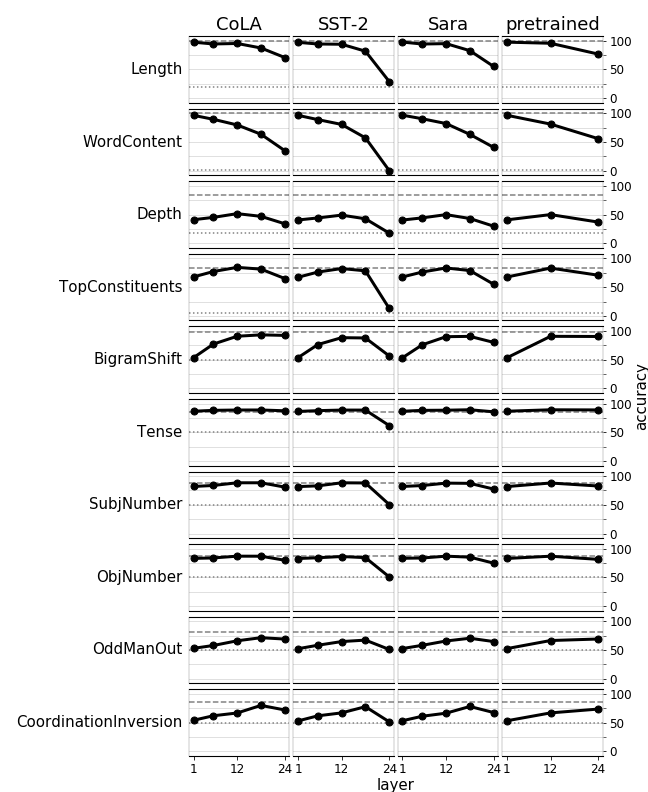
\includegraphics[width=12.5cm]{graphics/probing_master.png}
      \caption{Probing the 3 finetuned teachers and the pre-trained one. The dotted line shows baseline accuracy levels achieved by majority-class guessing, the dashed line shows human performance.}
      \label{fig:probing-master}
    \end{figure}
  }
}

\chapter{Overall discussion and conclusions}{}

\chapter{Future work}{}

\chapter{Plan for the rest of the semester}{
  Work finished:
  \begin{itemize}
    \item implementing everything related to distillation (incl. teacher finetuning and generating augmentation data with GPT-2)
    \item creating augmented transfer sets and finetuning the BERT teacher for each task
    \item exploring the model parameters shared across tasks (i.e. doesn't include embedding type and student size)
    \item implementing everything needed for probing
    \item implementing everything needed for gathering predictions for mistake/confidence analysis
  \end{itemize}

  Work to be done:
  \begin{itemize}
    \item now-Feb 10: finishing size exploration for SST-2 and Sara (ending up with best students for each downstream task)
    \item Feb 11-23: analysing the predictions of all models (includes Inovative Learning Week Feb 17-21 when I won't get terribly much done)
    \item Feb 11-16: probing the best students
    \item Feb 24-Mar 1: putting together overall analysis and conclusions
    \item Mar 2-Apr 2: buffer time and writing the report (a lot of coursework in this period as well)
  \end{itemize}
}

\bibliographystyle{apalike}
\bibliography{s1513472-minf2}

\appendix

\end{document}
